\documentclass[journal,transmag]{IEEEtran}

\usepackage{amsmath}
\usepackage{amssymb}
\usepackage{graphicx}
\usepackage{algpseudocode}
\usepackage{algorithm}
\usepackage{subfigure}
\usepackage{booktabs}
\usepackage{url}
\usepackage{breakurl}
\usepackage[breaklinks]{hyperref}

\begin{document}

\def\UrlBreaks{\do\/\do-}

%
% paper title
% Titles are generally capitalized except for words such as a, an, and, as,
% at, but, by, for, in, nor, of, on, or, the, to and up, which are usually
% not capitalized unless they are the first or last word of the title.
% Linebreaks \\ can be used within to get better formatting as desired.
% Do not put math or special symbols in the title.
\title{CS24110 Assignment: Automatic Enhancement of Digital Images via Automatic Contrast Adjustment on RGB, Histogram Equalisation on LAB Colour Space, and Average Value Blur Filter}


% author names and affiliations
% transmag papers use the long conference author name format.

\author{\IEEEauthorblockN{Dimitar Tasev}
\IEEEauthorblockA{Department of Computer Science, Aberystwyth University, Aberystwyth, SY23 3DB, UK}}% <-this % stops an unwanted space

% The paper headers
\markboth{CS24110}%
{D. Tasev}

\IEEEtitleabstractindextext{%
	
% Your abstract goes in here
\begin{abstract}
	This paper presents an approach to image enhancement, which combines multiple operations on the image, Automatic Contrast Adjustment, Luminosity Histogram Equalisation and Average Value Blur filter. This algorithm is hard to implement, and is expensive to compute, because there are multiple operations on the image, performed in sequence. The algorithm is tested on five test images and the results show that it can fix contrast and brightness issues, and improve the quality of the image. However, in some circumstances the results may not be satisfactory. These aspects are discussed in this paper.
\end{abstract}

}

% make the title area
\maketitle

\IEEEdisplaynontitleabstractindextext

\section{Introduction}

% The very first letter is a 2 line initial drop letter followed
% by the rest of the first word in caps.
% 
% form to use if the first word consists of a single letter:
% \IEEEPARstart{A}{demo} file is ....
% 
% form to use if you need the single drop letter followed by
% normal text (unknown if ever used by IEEE):
% \IEEEPARstart{A}{}demo file is ....
% 
% Some journals put the first two words in caps:
% \IEEEPARstart{T}{his demo} file is ....
% 
% Here we have the typical use of a "T" for an initial drop letter
% and "HIS" in caps to complete the first word.

\IEEEPARstart{T}{he} image enhancement to meet human visual perception is an important issue in general image processing, coding, machine vision. Nowadays, image enhancement is also widely adopted for medical image processing, texture synthesis, and speech recognition\cite{introQuote}. Image enhancement in computer graphics, the process of improving the quality of a digitally stored image by manipulating the image with software. It is quite easy, for example, to make an image lighter or darker, or to increase or decrease contrast. Advanced image enhancement software also supports many filters for altering images in various ways\cite{quoteImageEnhancement}.
Image editing encompasses the processes of altering images, whether they are digital photographs, traditional photochemical photographs, or illustrations. Traditional analog image editing is known as photo retouching, using tools such as an airbrush to modify photographs, or editing illustrations with any traditional art medium. Graphic software programs, such as Adobe\textsuperscript{\texttrademark} Photoshop\textsuperscript{\textregistered} and GIMP\footnote{\url{http://www.gimp.org}}, are the primary tools with which a user may manipulate, enhance, and transform images. Many image editing programs are also used to render or create computer art from scratch.\

The problem presented is to create an algorithm for automatic image enhancement. The area has been developing recently, the biggest contributor being the creation of Instagram\textsuperscript{\texttrademark}, and the filters that they use to automatically enhance pictures, which have become very popular. Another popular automatic enhancement application is Google Photos \footnote{\url{https://photos.google.com/}}, also providing a variety of filters, and automatic picture enhancement. 

This paper is concerned with a new method to enhance a given image. The idea behind the approach is to merge the effects of three different operations, Automatic Contrast Adjustment, Luminosity Histogram Equalisation and Average Value Blur filter, each acting on a different area of the picture. In theory this should correct any contrast issues, any brightness issues, and remove noise artefacts, if such are available.

In this paper the methodology for the proposed image enhancement algorithm will be given at both high and low level in Section \ref{sec:methods}. The results are shown in Section \ref{sec:results} and then discussions and conclusion are drawn in Section \ref{sec:discussion}.

\begin{figure}[h!]
\centering
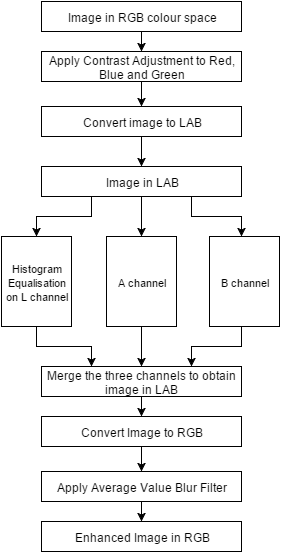
\includegraphics[width=0.42\textwidth]{figures/flowchart.png}
\caption{A flowchart of the proposed enhancement method. It shows the steps that will be performed in the automatic enhancement.}
\label{fig:flowchart}
\end{figure}

\section{Methodology}
\label{sec:methods}

% Blur Filter >
%  RGB TO LAB, 
% Histogram Equalisation, 
% Lab to RGB, 
% Contrast Adjustment
In this section the methods behind the Average Value Blur Filter, Colour Space Conversion, Histogram Equalisation, and Contrast Adjustment is described. A high-level overview of how the method works, a mathematical outline and pseudocode are also provided.
%In this section the methodology behind the mean matching approach to image enhancement is described.  As well as a high-level overview of how the method works, a mathematical outline and pseudocode are also provided.

\subsection{High-level Overview}
The idea behind the proposed automatic enhancement approach is to do a contrast adjustment to remap the intensity value so that the whole range of possible values is used, convert to LAB(CIELAB) colour space and perform a Histogram Equalisation on the Luminosity channel to enhance the picture\cite{labHistEqArticle}, then convert back to RGB, and apply an Average Value Blur Filter for noise removal. The enhancement will follow the flowchart on Figure \ref{fig:flowchart}.

\begin{figure}[h!]
\centering
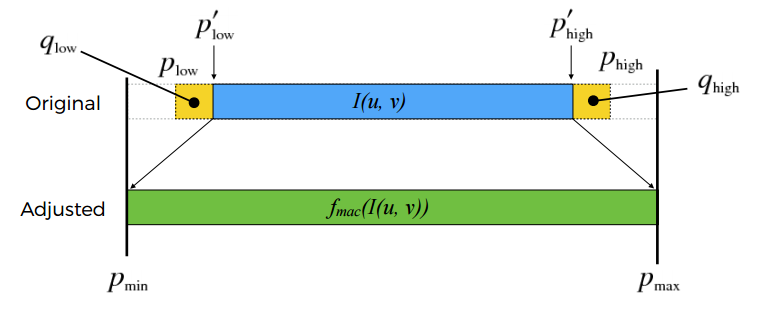
\includegraphics[width=0.42\textwidth]{figures/contrAdj.png}
\caption{An image showing how the range of values will be set when applying contrast adjustment to the picture.}
\label{fig:contrAdj}
\end{figure}

\begin{algorithm}[bh!] %normal hist
	\caption{Normal Histogram}
	\label{alg:norm_hist}
	\begin{algorithmic}[1]
		\Function{NormalHistogram} {$I$}\Comment{where $| I | = m \times n$, \\ $K = $ MAX value of the colour space, 256 for RGB, 101 for LAB's L channel}
		\State
		\State $H = [0, K-1]$
		\State 
		\For{\textbf{each} $p$ \textbf{in} $I$} 
		\State $H(p) = H(p) + 1$
		\EndFor
		\State 
		\State
		\Return $H$
		\EndFunction
	\end{algorithmic}
\end{algorithm}
\begin{algorithm}[bh!]%cumulative hist
	\caption{Cumulative Histogram}
	\label{alg:cum_hist}
	\begin{algorithmic}[1]
		\Function{CumulativeHistogram} {$I$}\\ \Comment{where $K = $ MAX value of the colour space, 256 for RGB, 101 for LAB's L channel}
		\State
		\State $H = $ NormalHistogram()
		\State $CH = [0, K-1]$
		\State
		\For{\textbf{each} $v$ \textbf{in} $H$} 
		\State $CH[v] = CH[v-1] + H[v]$
		\EndFor
		\State 
		\State
		\Return $CH$
		\EndFunction
	\end{algorithmic}
\end{algorithm}

\subsection{Detailed Description}
The proposed enhancement method is a combination of filter and point-based histogram operations. To simplify the description of the operations, the algorithms assume that the picture is grayscale, however the final algorithms work on RGB images, by repeating the functions for each colour channel. 
\begin{figure}[h!] % normal and cumulative histograms 
	\centering
	\subfigure[original] {
		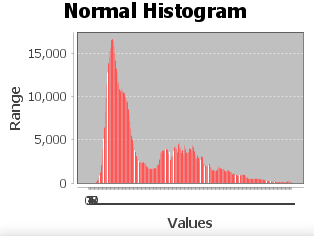
\includegraphics[width=0.2\textwidth]{figures/norm_hist.png}
	}
	\subfigure[modified] {
		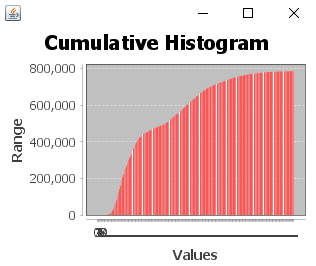
\includegraphics[width=0.2\textwidth]{figures/cum_hist.png}
	}
	\caption{Two images showing a normal histogram and a cumulative histogram of it.}
	\label{fig:hist_comp}
\end{figure}
The first two operations both rely on histograms to perform their operations. A histogram is a graphical representation of a distribution of numerical data\cite{histDesc}\cite{histDescWiki}. In this paper the histograms are created using \textit{JFreeChart}\cite{jFreeChart}. Figure \ref{fig:hist_comp} shows both a normal histogram and a cumulative histogram, both of which are used. The pseudocode for creating a \textbf{normal histogram} \ref{alg:norm_hist}, and the pseudocode for creating a \textbf{cumulative histogram} from the normal histogram \ref{alg:cum_hist} are included in the paper. The equation for deriving a cumulative histogram from a normal histogram can be simply written as: 

\begin{equation}%equation for cumulative histogram
\begin{aligned}
H(i) &=  \sum_{j = 0}^{i}h(j) 
& for(0 \leq i < K)
\end{aligned}
\end{equation}
\begin{figure}[t] % normal and contrast adjusted histograms 
	\centering
	\subfigure[original] {
		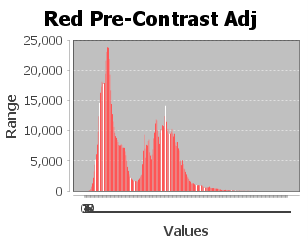
\includegraphics[width=0.2\textwidth]{figures/pre_contr_adj.png}
	}
	\subfigure[modified] {
		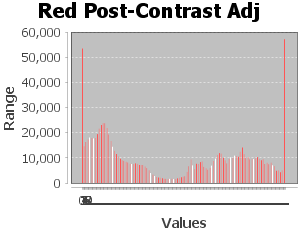
\includegraphics[width=0.2\textwidth]{figures/post_contr_adj.png}
	}
	\caption{Two images showing a normal histogram before and after being contrast adjusted.}
	\label{fig:contrAdjustedHist}
\end{figure}

The first operation, the Contrast Adjustment, is performed on the image in RGB colour space, so no conversion is needed. In images often the full range of values isn't used. Automatic contrast adjustment remaps the intensity values so that they occupy the full range of possible values\cite{automaticContrast}. We have to identify two quantiles at the low $p'_{low}$ and high $p'_{high}$ end of the intensity spectrum, and map the pixel values inside them to the extreme values, the other pixels are then linearly mapped to the interval [$p_{min}, p_{max}$] as seen on Figure \ref{fig:contrAdj}. To calculate the two quantiles we set a range for ignored pixels $q$. Using that range we can calculate the quantiles using the cumulative histogram:

\begin{equation} %equation for getting the P value for contr adjustment
\begin{aligned}\label{eq:contrAdjPlowNPhigh}
&p'_{low} = \min\{i \text{ } | \text{ } CH(i) \geq m\cdot n \cdot q_{low}\}\\
&p'_{high} = \max\{i \text{ } | \text{ } CH(h) \leq m\cdot n \cdot q_{high}\}
\end{aligned}
\end{equation}

\noindent Given that q follows: 
\begin{equation}\label{eq:contrAdjQcalc}
0 \leq q_{low}, q_{high} \leq 1, q_{low} + q_{high} \leq 1
\end{equation}

\noindent After applying the formula to the cumulative histogram we will get ranges, which can be visually represented like this:
\begin{center}
	 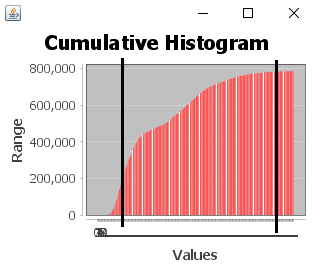
\includegraphics[width=0.2\textwidth]{figures/cum_hist_range.png}
	 \label{fig:cumulativeHistRange}
\end{center}
Then we loop through the pixels in the picture and apply the following function $f$ to each pixel: 

\begin{center}
	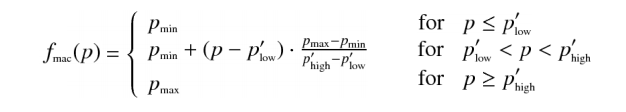
\includegraphics[width=0.5\textwidth]{figures/contrAdjFormula.png}
	\label{fig:contrAdjFunc}
\end{center}

\noindent We can see the difference in the histograms after adjusting the contrast \ref{fig:contrAdjustedHist}, the value range now occupies the whole spectrum of possible intensities.
%\begin{equation}
%\begin{aligned}
%\[
%	f(x) = 
%	\begin{cases}
%	p_{min}, &\text{for } p \leq p'_{low}\\
%	p_{min} + (p - p'_{low})\cdot \frac{p_{max}-p_{min}}{p'_{high}-p'{low}}, &\text{for } p'_{low} < p < p'_{high}\\
%	p_{max}, &\text{for } p \geq p'_{high}
%	\end{cases}
	
%\]
%\end{aligned}
%\end{equation}


The second operation of the algorithm is Histogram Equalisation on the Luminosity channel in LAB(CIELAB) colour space. It adjusts the contrast and brightness to appear as they would in a well exposed picture. As we can see in Figure \ref{fig:luminDiffHist}, if the brightness of the picture is low, i.e. the picture is dim, the Luminosity channel is concentrated in the lower end of the spectrum. If the picture is bright, it is concentrated in the high end of the spectrum. In order to equalise the Luminosity channel, we first have to convert the image to LAB. This cannot be done directly, so the RGB picture has to be converted to XYZ colour\cite{rgbTOxyz} space first, and then converted to LAB\cite{xyzTOlab}. Then a normal and cumulative histograms have to be created on the Luminosity (L) channel, using the methods described earlier \ref{alg:norm_hist}, \ref{alg:cum_hist}. From the cumulative histogram we can equalise the pixel distribution, so that the histogram of the image approximates a uniform distribution. The goal of histogram equalisation is to shift the pixels in the image, so that the resulting cumulative histogram is approximately linear. \cite{automaticContrast} Figure \ref{fig:equal_hist} is showing the cumulative histogram of the L channel before equalisation, and after equalisation. Histogram equalisation on the cumulative histogram is done using algorithm \ref{alg:equal_hist}, implementing the following equation: 
\begin{equation}
f_{he}(p) = \lfloor CH(p) \cdot \frac{K - 1}{mn}\rfloor
\end{equation}
\noindent After the Equalised Histogram has been created, we have to loop through each pixel in the image and set its new value, which is stored in the Equalised Histogram, at the position of the pixel's current value: 
\begin{equation}\label{eq:histEqPixel}
P(v) = EQH(P(v))
\end{equation}
\begin{algorithm}[h!] %histogram equalisation
	\caption{Histogram Equalisation}
	\label{alg:equal_hist}
	\begin{algorithmic}[1]
		\Function{HistogramEqualisation} {$I$}\\ \Comment{where $K = $ MAX value of the colour space, 256 for RGB, 101 for LAB's L channel}
		\State
		\State $CH =$ CumulativeHistogram(I)
		\State $EQH = [0, K-1]$
		\State
		\For{\textbf{each} $v$ \textbf{in} $CH$} 
		\State $EQH(v) = CH(v)\cdot\frac{K-1}{m \times n}$
		\EndFor
		\State 
		\State
		\Return $EQH$
		\EndFunction
	\end{algorithmic}
\end{algorithm}
\begin{figure}
		\centering
		\subfigure[original] {
			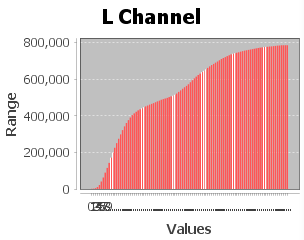
\includegraphics[width=0.2\textwidth]{figures/cum_labhist.png}
		}
		\subfigure[modified] {
			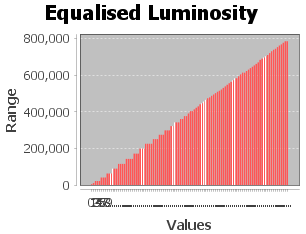
\includegraphics[width=0.2\textwidth]{figures/equal_labhist.png}
		}
		\caption{Two images showing a normal histogram and the equalised histogram of it.}
		\label{fig:equal_hist}
\end{figure}
%TODO colour space conversion pseudocode

The last operation in the algorithm, the Average Value Blur is a filter, because it does not rely solely on a single pixel's value. The filter loops through the picture and acts on each pixel, but in the calculation the values of the neighbouring pixels are also included. Its effect is to reduce the noise in the picture, by applying a blur effect.\cite{averageFilter} The strength of the blur, however, heavily depends on the size of the picture. Small pictures (i.e. 640x480 resolution) will have very strong blur, to the point of ruining the picture, and very big pictures (i.e. 1920x1020 resolution) will have nearly no visible change. The described filter operation acts on each channel in the same manner, using a filter operation function $f$. That is: 
%TODO add pseudo code for filter operation? 

\begin{equation}\label{eq:avgFilter} %equation that shows filter calculation
I'(u, v) = f(\frac{1}{9}\cdot\sum_{j=-1}^{1}\sum_{i=-1}^{1}I(u+i, v+j))
\end{equation}

\subsection{Implementation}
The detailed description section focuses on a single colour channel; however, since the algorithm needs to work on RGB images, the above methods needs to be repeated for each of the colour channels. The three enhancement operations are used in sequence in the image enhancement algorithm. Each of them will be looked at separately, in the order that they are applied in the algorithm, because if the order is changed, the final result will also be different. At the end of each of the operations, a clamping operation will be used to ensure that the modified intensities do not fall out of the displayable range.

The first operation is \textbf{Automatic Contrast Adjustment} on the RGB channel. To achieve that the implementation will create and store a Normal Histogram \ref{alg:norm_hist} for each of the channels. When the Normal Histograms have been calculated, we can use them to create the Cumulative Histograms \ref{alg:cum_hist}, repeated for each of the channels. Then we have to pick appropriate $q_{low}$ and $q_{high}$, following the equation \ref{eq:contrAdjQcalc}. Now we can calculate $p'_{low}$ and $p'_{high}$ for each of the colour channels using the Cumulative Histograms of the channels \ref{eq:contrAdjPlowNPhigh}. After we have calculated $p'_{low}$ and $p'_{high}$, we apply the function \ref{fig:contrAdjFunc} to each pixel to determine it's new value. After the Contrast Adjusted image is produced, we perform the second operation from the algorithm, the Luminosity Histogram Equalisation.

In order to create a \textbf{histogram} on the \textbf{Luminosity channel}, we have to convert each pixel to LAB colour space, before performing any operations. As this cannot be done directly from RGB, we first need to convert it into XYZ \cite{rgbTOxyz} colour space, and then into LAB \cite{xyzTOlab} colour space. The implementation has to loop through each pixel, converting it to LAB colour space, and creating a Normal Histogram \ref{alg:norm_hist} of the Luminosity (L channel for short). When the Normal Histogram is calculated, a Cumulative Histogram \ref{alg:cum_hist} is created from it, and finally an equalisation \ref{alg:equal_hist} is performed on the Cumulative Histogram. After the Equalised Histogram has been completed, the implementation loops through all of the pixels, converting each one to LAB, and then adjusts the intensities \ref{eq:histEqPixel}, using the new values from the Equalised Histogram. When the pixels' values are adjusted, the implementation has to convert the pixel from LAB back to XYZ \cite{labTOxyz}, and then to RGB \cite{xyzTOrgb}. A clamping operation is performed as well, before finally setting the new value of the pixel.

The last operation performed by the enhancement algorithm is the \textbf{Average Value Blur} filter. It works in RGB colour space, so it does not need to convert the picture. The filter is easy to implement, it calculates the average value of the pixel, plus the surrounding pixels \ref{eq:avgFilter}. After it loops through every pixel, a blurred image is produced, which is also the final product image of the algorithm.

This Image Enhancement algorithm is very expensive to compute, and will be visibly slow when executed on older computers. It's implementation can be optimised by using an efficient pixel accessing mechanism, such as Java's \textit{WritableRaster}, but it's run time will still be noticeably long. This is due to combining multiple operations, each of them acting on the \textit{whole} image, in sequence.

\begin{figure*}[t]
	\centering
	\subfigure[Image 1 Original]{
		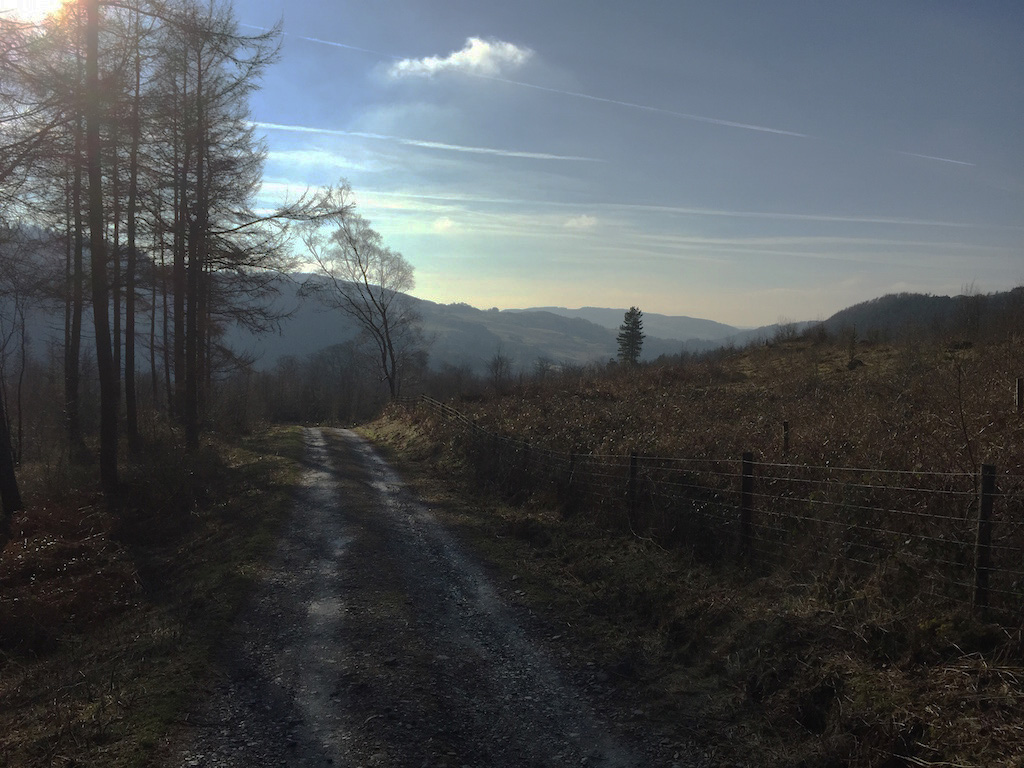
\includegraphics[width=0.225\textwidth]{figures//images//image_01.jpg}
	}
	\subfigure[Image 1 Modified]{
		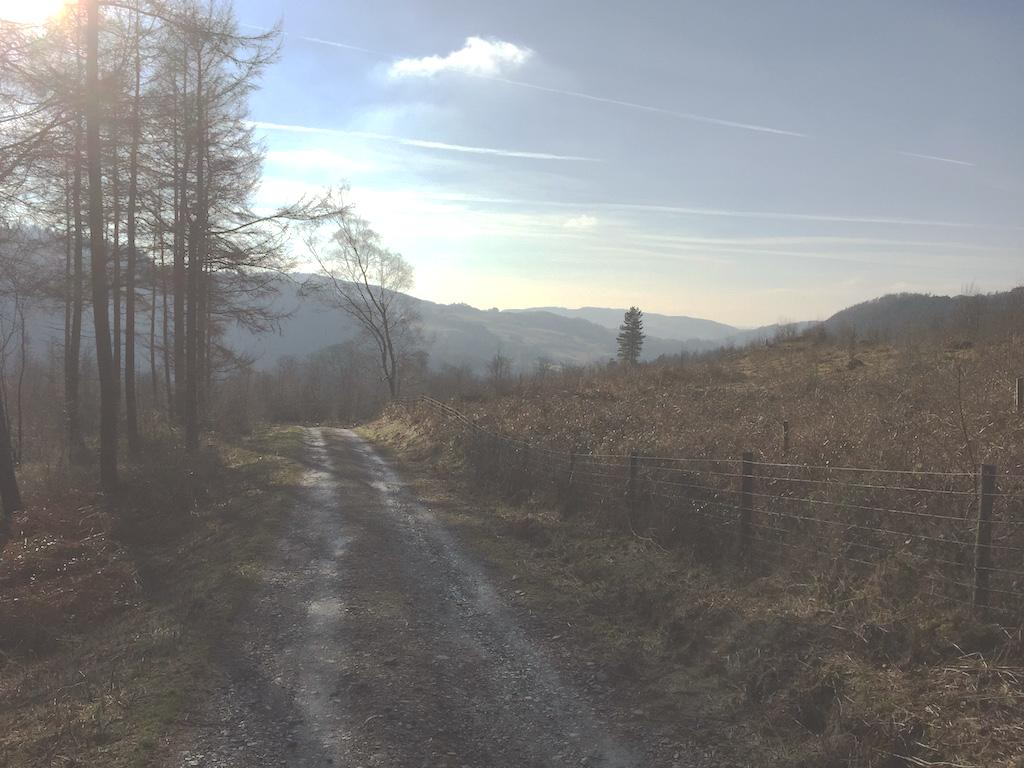
\includegraphics[width=0.225\textwidth]{figures//images//image_01_changed.jpg}
	} 
	\subfigure[Image 2 Original]{
		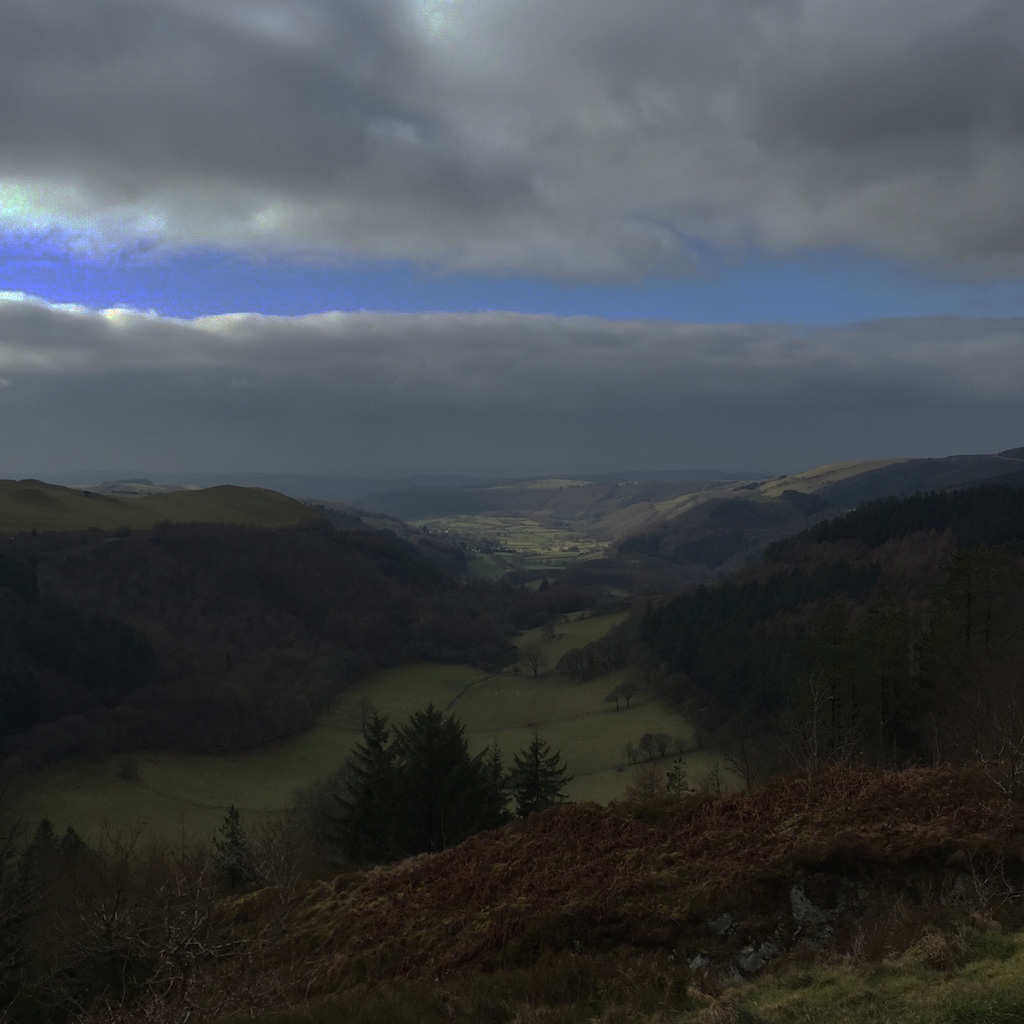
\includegraphics[width=0.225\textwidth]{figures//images//image_02.jpg}
	}
	\subfigure[Image 2 Modified]{
		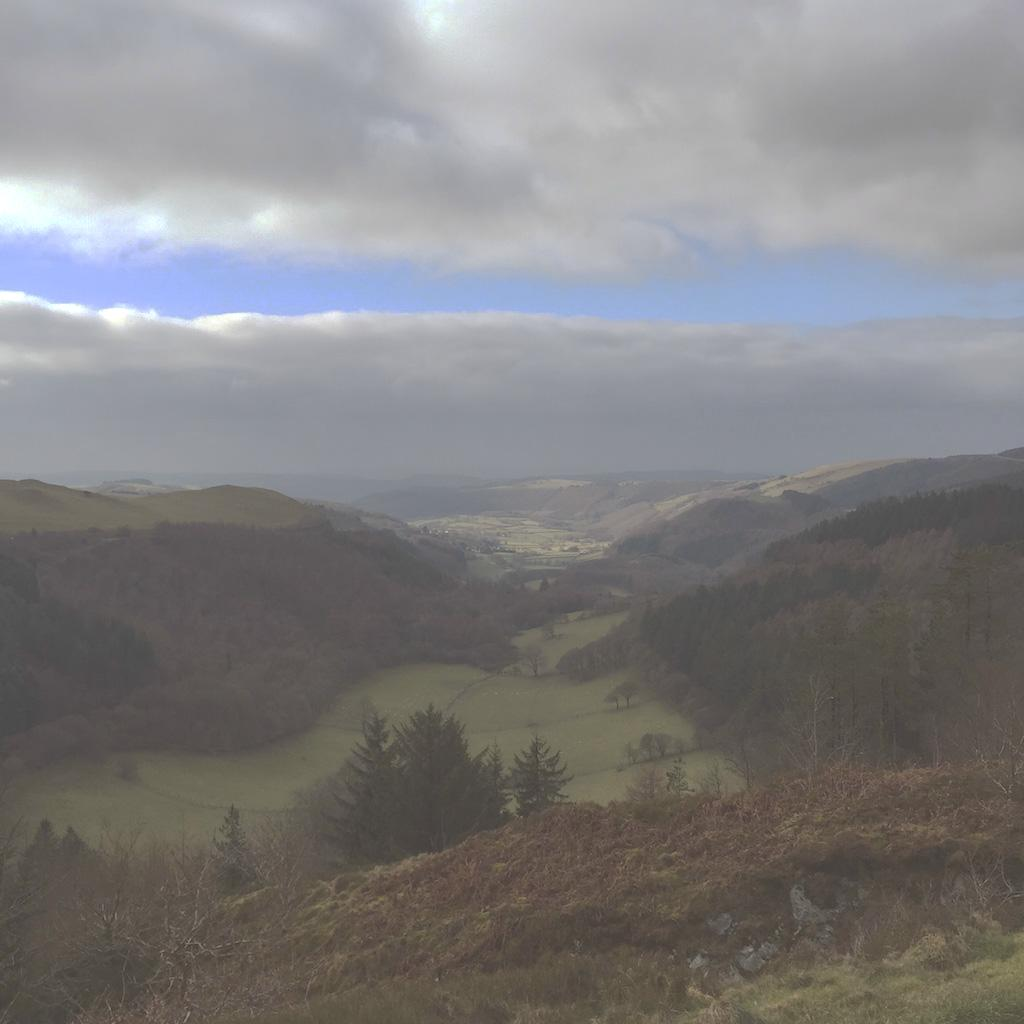
\includegraphics[width=0.225\textwidth]{figures//images//image_02_changed.jpg}
	} \\
	\subfigure[Image 3 Original]{
		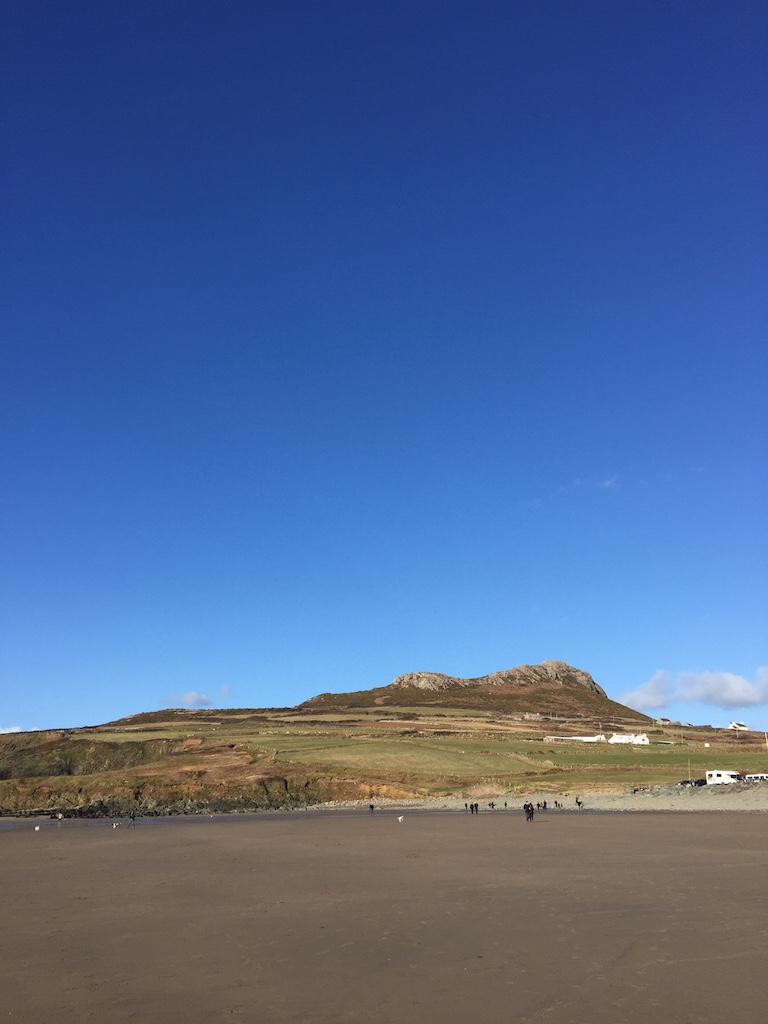
\includegraphics[width=0.225\textwidth]{figures//images//image_03.jpg}
	}
	\subfigure[Image 3 Modified]{
		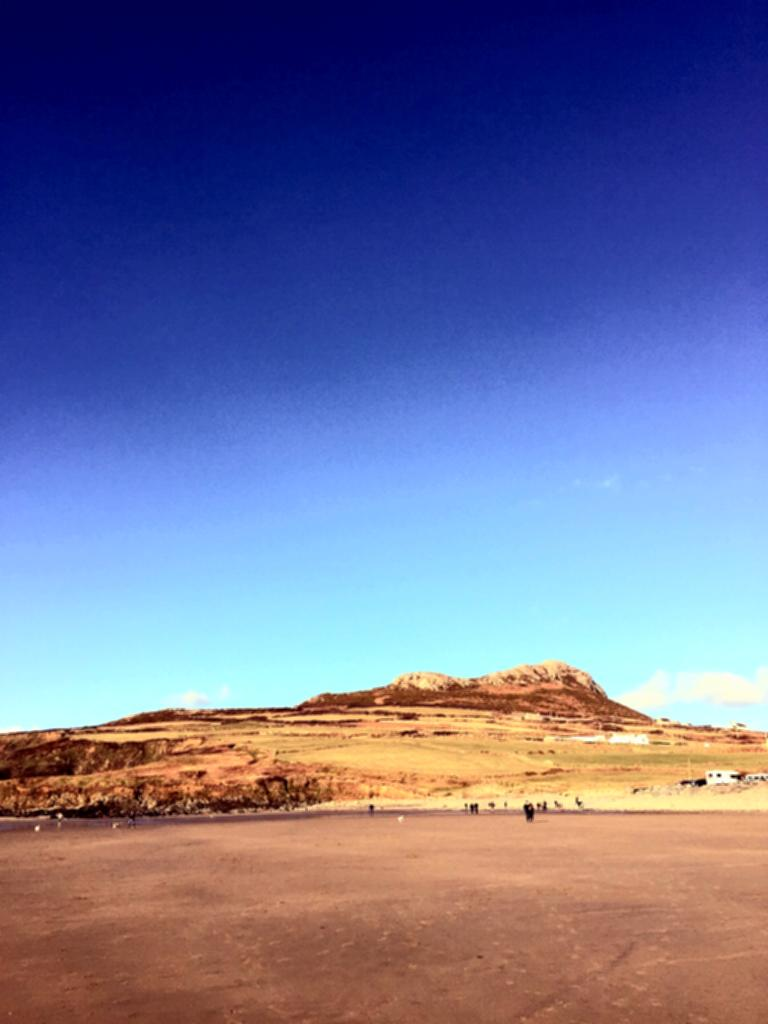
\includegraphics[width=0.225\textwidth]{figures//images//image_03_changed.jpg}
	} 
	\subfigure[Image 4 Original]{
		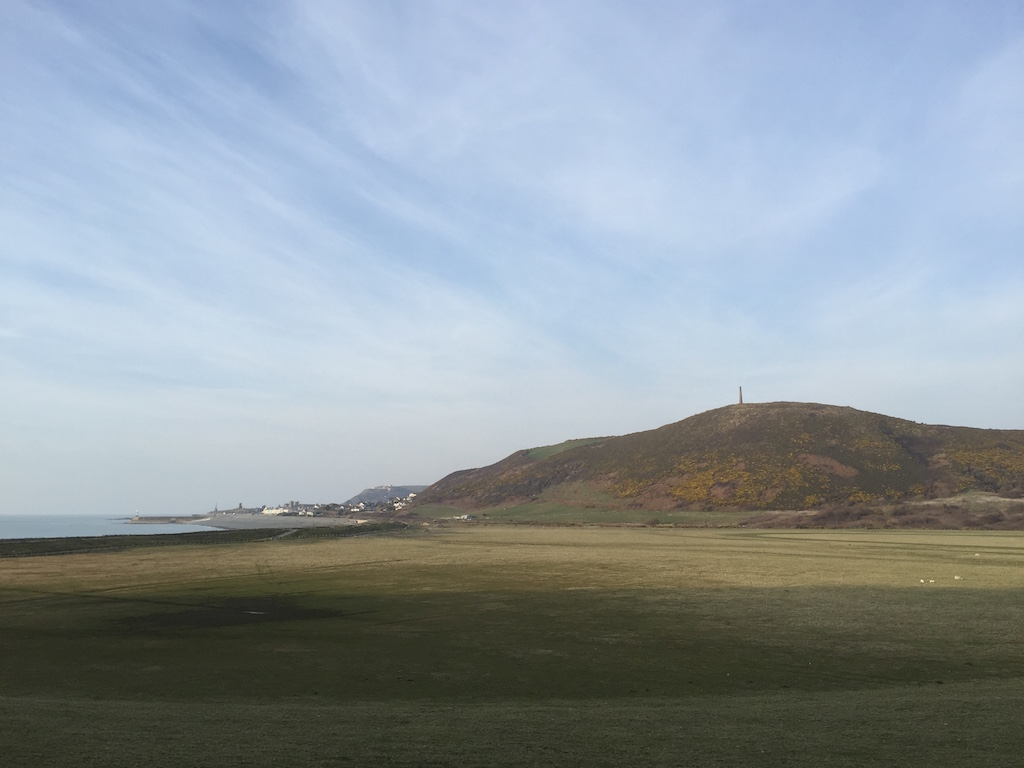
\includegraphics[width=0.225\textwidth]{figures//images//image_04.jpg}
	}
	\subfigure[Image 4 Modified]{
		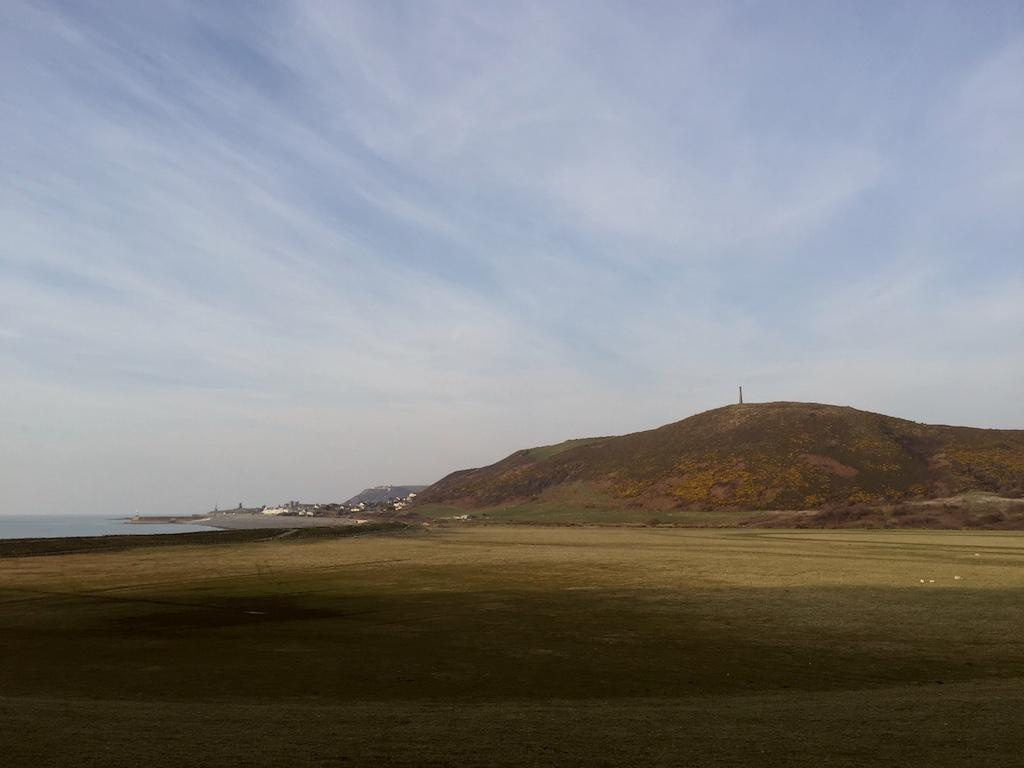
\includegraphics[width=0.225\textwidth]{figures//images//image_04_changed.jpg}
	} \\
	\subfigure[Image 5 Original]{
		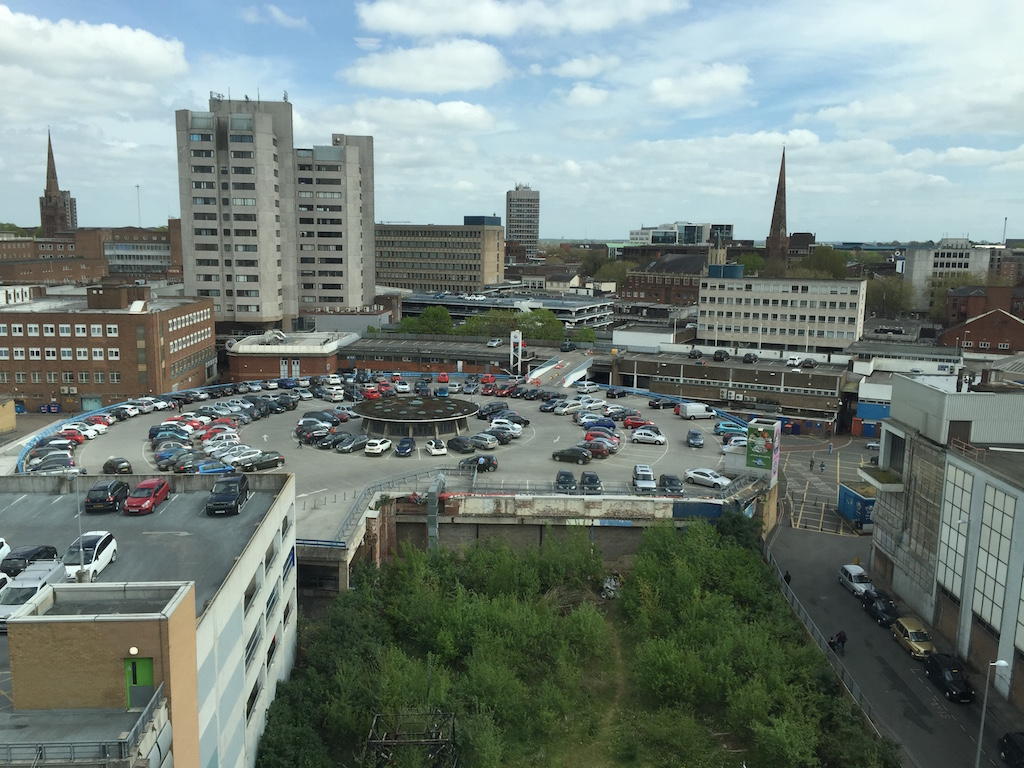
\includegraphics[width=0.225\textwidth]{figures//images//image_05.jpg}
	}
	\subfigure[Image 5 Modified]{
		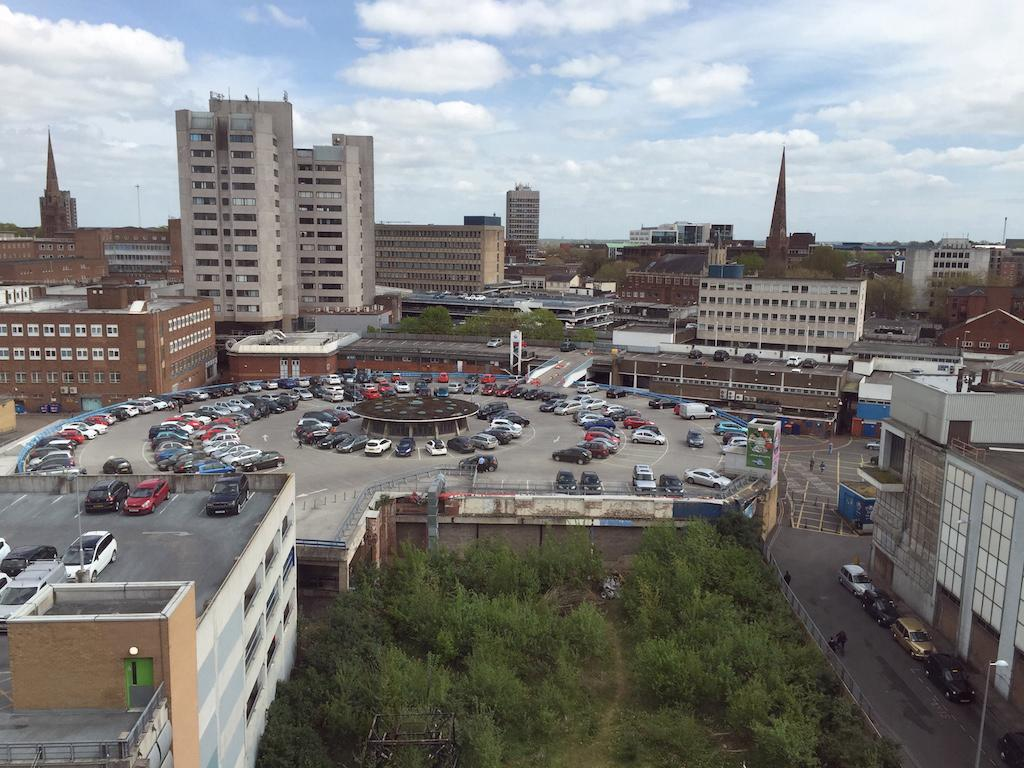
\includegraphics[width=0.225\textwidth]{figures//images//image_05_changed.jpg}
	} \\
\caption{Results of performing the mean alignment algorithm on each of the five test images.  For the first two images (a, c), the algorithm produces washed out results (b, d).  Performing the algorithm on Image 3 (e) causes a drastic change in colour (f), whereas the results for Image 4 (g) are far more natural (h).  The effect of the algorithm is least noticeable on Image 5 (i, j). 
	Results of performing the described image enhancement algorithm on each of the five test images. The effect of the algorithm is noticeable in all of the images, they are all brighter and the blur is visible. For images (e, g) the images produced do not look natural (f, h). The algorithm's effect on image (a) has brought in colours in the sky that are not in the original picture (b). For images (c, i) the algorithm produced more natural-looking results. }
\label{fig:results}
\end{figure*}

\begin{figure}[h!]
	\centering
	\subfigure[original] {
		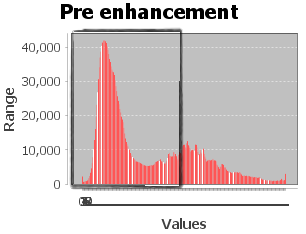
\includegraphics[width=0.2\textwidth]{figures/image_01_pre_enh_combined_hist.png}
	}
	\subfigure[modified] {
		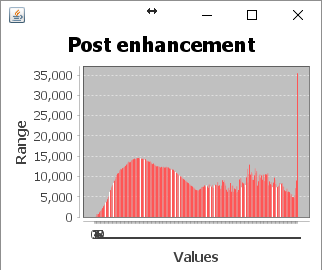
\includegraphics[width=0.2\textwidth]{figures/image_01_post_enh_combined_hist.png}
	}
\caption{Average RGB histograms from image 1 (Figure \ref{fig:results} (a, b)).  The unnatural colours occurs, because the original pixel intensity distribution is mostly focused in a particular range, surrounded by a black square, but after contrast adjustment the full range is used, bringing out unnatural colours.}
\label{fig:image01_hists}
\end{figure}

\begin{figure}[h!]
	\centering
	\subfigure[low brightness] {
		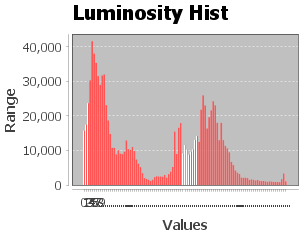
\includegraphics[width=0.2\textwidth]{figures/low_brightness_hist.png}
	}
	\subfigure[high brightness] {
		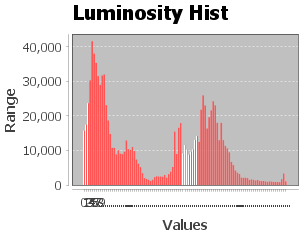
\includegraphics[width=0.2\textwidth]{figures/high_brightness_hist.png}
	}
	\caption{Luminosity channel histograms of a low brightness picture (left) and high brightness picture (right).}
	\label{fig:luminDiffHist}
\end{figure}

\section{Results}
\label{sec:results}
The proposed image enhancement method is tested on the five provided images. The results of performing the algorithm are shown in Figure \ref{fig:results}.

The image enhancement algorithm causes a change in all of the images. 
The least change is seen in Image 5 (Figure \ref{fig:results} (i, j)). The most natural looking images are Image 2 and Image 5; in the rest of the images there are large colour changes, bringing out unnatural colours. The blur from the filter is noticeable in all of the images.

The modified version of Images 1, 3 and 4, all have unnatural colours appear. This is due to the Automatic Contrast Adjustment remapping the images to use all of the available intensities, when the original picture pixels' intensity was mostly concentrated on a particular range. This can be seen when looking at the histograms. Figure \ref{fig:luminDiffHist} shows the histogram before and after processing Image 1. We can see how before the algorithm, the image's pixel intensity values were focused mostly in a particular range, but after being processed by the algorithm, they are spread out, bringing out colours, that would not be very well visible in the original picture.

The second operation in the algorithm, the Histogram Equalisation on the Luminosity channel, is responsible for the pictures looking clearer than the original, and the brightness change that can be seen in all of them. Images 1 and 2 have had their brightness increased after being processed, due to the original picture being dim. Images 4 and 5, have only a slight difference from the original picture's brightness. However, since they appear to be a bit washed out in the original pictures, after equalisation it can be see that they are clearer and less washed out. The same effect appears on Image 3, but it is weaker. Images 3, 4 and 5 have not been significantly changed by the Luminosity channel Histogram Equalisation, because the original pictures are fairly well exposed and have good brightness.

The final operation in the algorithm, the Average Value Blur filter is responsible for the visible blur in the pictures. The blur might be a little bit too strong than desirable, because the pictures are small in size.

\section{Discussion \& Conclusions}
\label{sec:discussion}

The results show that the proposed method works best when the picture isn't heavily focused on one colour, causing the Automatic Contrast Adjustment to bring out unnatural colours, that are not seen in the original pictures. If pictures appear to be dim, or washed out, the method will adjust them to appear as if they were well exposed, brighter/less washed out. 
The Average Value Blur filter can be very strong on small pictures, reducing their quality rather than enhancing it, and unnoticeable on large pictures, making it rather unnecessary. The picture sizes are small, that is why the blur effect is a bit stronger than what would be optimal.

From that we can conclude that the algorithm works well with pictures that do not have a single dominating colour. If the pictures happen to be underexposed and appear to be dim or overexposed and washed out, the method will work well, and will properly adjust them. However having the Average Blue Filter's usefulness depend on the picture size is impractical. 

An improvement for the algorithm would be to add a different blur filter one which is consistent and independent of picture size. Also it would be beneficial to try and find a way to avoid the unnatural colours from the Automatic Contrast Adjustment. Adding an edge enhancement operation, which will sharpen the picture might also be beneficial for this image enhancement algorithm. %TODO add what more can be improved? //more??!?
\\
\\
In conclusion, this paper has presented a method for automatic image enhancement, incorporating multiple image enhancement operations, each acting on a different area of the picture, with one of the operations being performed in a different colour space. This makes it a hard algorithm to implement, and expensive to execute, as it has multiple operations, histograms and colour space conversions, all of which are necessary parts to make the algorithm work. In some cases the algorithm is able to improve the quality of the picture, adjusting the brightness to imitate a well exposed picture, good contrast range using all of the possible values and reducing the noise of the picture. However, in other cases the contrast adjustment can bring out unwanted unnatural colours, that are not visible in the original picture. The strength of the Average Value Blur filter is also of concern, because having the strength depend on the size of the picture is impractical.

% can use a bibliography generated by BibTeX as a .bbl file
% BibTeX documentation can be easily obtained at:
% http://www.ctan.org/tex-archive/biblio/bibtex/contrib/doc/
% The IEEEtran BibTeX style support page is at:
% http://www.michaelshell.org/tex/ieeetran/bibtex/
\bibliographystyle{IEEEtran}
% argument is your BibTeX string definitions and bibliography database(s)
\bibliography{biblio}


% if you will not have a photo at all:
% that's all folks
\end{document}


